\section{Live-Migration als Teil der Lösung}
\label{sec:livemigration}
Hansen präsentierte das
NomadBIOS~\cite{nomadbioslivemigration-cloudseminar} als
Live-Migrations-Lösung als Teil der Lösung für oben genannte Probleme
der Clouds. Im Folgenden werden wir auf die von ihm vorgestellte
Lösung technische rekapitulieren und dabei den Lösungsbeitrag
aufzeigen.

\subsection{Verlässlichkeit von Virtualisierung}
In jedem verteilten System muss man mit der Realität umgehen, dass
Hardware und Software Fehler enthält, die zu Ausfällen führen
können. Da scheint die Idee, viele Virtuelle Maschinen auf wenigen
physikalischen Systemen auszuführen zunächst wie ein Schritt in die
falsche Richtung: Wenn dann ein physikalischer Server ausfällt, oder
die Virtualisierungssoftware einen Fehler enthält, fallen potentiell
eine ganze Reihe von Diensten auf einmal aus. In der Realität
entstehen die meisten Fehler in Datencentern allerdings durch
Softwarefehler~\cite{tanenbaum1992modern}. Softwarefehler können umso
häufiger zutage treten, je mehr unterschiedliche Systeme miteinander
interagieren müssen, und je größer die Code-Basis der einzelnen
Systeme ist~\cite{zellerprograms}. Durch Virtualisierung kann man
Softwaresysteme voneinander isolieren, ohne für jedes System einen
eigenen, physikalischen Server mit eigenem Betriebssystem
bereitzustellen. Der Hypervisor selbst ist in solch einem Fall die
einzige Software, die im Kernel Modus läuft, und dieser hat um
Größenordnungen weniger Zeilen Quelltext als ein aktuelles
Betriebssystem~\cite{tanenbaum1992modern}. Folglich enthält der
Hypervisor wahrscheinlich weniger Bugs~\cite{zellerprograms}.

Kritische Dienste können so in kompletter Isolation ausgeführt um das
Risiko eines Ausfalls durch inkompatible Software auf demselben Server
zu minimieren.

Nichtsdestotrotz müssen auch Vorkehrungen gegen Hardwarefehler
getroffen werden. In klassischen Hosting-Umgebungen kann man bei
immanenten Ausfällen von physikalischen Systemen relevante Prozesse
auf neue VMs migrieren~\cite{hansen2004self}. Für eine gegebene VM
kann eine Ähnliche (z.B. aus einem früheren, gesicherten Zustand) auf
einem neuen Server gestartet werden. Der Zustand der relevanten
Prozesse wird soweit als möglich gemäß den Gegebenheiten des
Betriebssystems kopiert und neue Dienstanfragen dann auf den neuen
Server umgeleitet. Die alte VM muss allerdings zunächst online
bleiben, um Abhängigkeiten von Dienstanfragen bereitzustellen, die
sich noch in Ausführung befinden, wenn der Hardwarealarm ausgelöst
wird~\cite{clark2005live}. Das ist bekannt als "`residual
dependencies problem"' (Problem mit verbleibenden Abhängigkeiten).

Diese Vorgehensweise zur Migration auf Prozessebene hat also den
wesentlichen Nachteil, dass laufende Prozesse nicht verschoben werden
können, sondern noch auf der bestehenden Hardware zum Ende laufen
müssen. Die meisten Applikationen verlassen sich auf viele
verschiedene Weisen auf die Fähigkeiten des Betriebsystems, die
Hardware anzusteueren und in geeignete Zustände zu überführen, die den
Ablauf der Applikation erst möglich machen. Das heißt, dass ein
laufender Prozess meistens nicht einzeln verschoben werden
kann~\cite{hansen2002nomadic}. Im Falle eines Web-Servers, bei dem
jeder Request auch an einen neuen Prozess gehen kann, ist das nicht
weiter problematisch. Schwieriger ist die Situation bei Diensten wie
z.B. Online-Spieleplattformen, bei denen ein Serverprozess
TCP-Verbindungen zu mehreren Clients teilweise über Stunden aufrecht
erhalten muss. Wenn ein Hardwareausfall kurz bevor steht, bleibt hier
meist nichts anderes übrig, als das Spiel zu unterbrechen: Das kann
bedeutet mindestens unzufriedene Kunden, und vielleicht sogar
verringerten Umsatz.

Wenn man aber stattdessen den Prozess und die virtuelle Maschine als
Einheit betrachtet~\cite{nelson2005fast}, und geschlossen live
migriert, kann auf Hardwarefehler angemessener reagiert werden: Zuerst
kann die VM bis aufs letzte Detail vom aktuellen Stand kopiert werden,
das heißt, dass Änderungen, die seit der letzten Checkpoint-Sicherung
geschehen sind, nicht verloren gehen. Wichtiger, allerdings, ist, dass
auch Prozesse, die sich gerade in Ausführung befinden, migriert werden
können. Im Beispiel der Spieleplattform bedeutet dies, dass Spiele
nicht unterbrochen werden müssen, sondern, für den Nutzer transparent,
auf den neuen Server migriert werden.

\subsection{Interoparibilität von Virtualisierungs-Lösungen}
Für Unternehmen, die mit öffentlichem Cloud-Hosting liebäugeln, kann
die Bindung an ein bestimmtes System schwerwiegende Konsequenzen nach
sich ziehen. Um mit der Flexibilität vom eigenen Rechenzentrum
mitzuhalten, darf die Virtualisierungstechnologie des Providers nicht
die Verwendung des Systems innerhalb das Unternehmens
einschränken. Insbesondere muss für den Kunden die Möglichkeit
bestehen, auf eine andere Virtualisierungstechnologie umzusteigen, um
z.B. vorhandene VMs auf die Technologie eines Cloud-Anbieters zu
bewegen oder umgekehrt auch VMs aus der Cloud wieder in das eigene
Rechenzentrum oder auf die Rechner der Entwickler umzuziehen. Die
Interoparibilität der verwendeten Virtualisierungslösungen spielt hier
eine wichtige Rolle.

Virtuelle Maschinen variieren stark zwischen verschiedenen
Virtualisierungslösungen. Das fängt mit den Formaten der virtuellen
Dateisysteme an und geht bis hinunter zu den spezifischen Arten der
virtualisierten Hardwarekomponenten~\cite{nelson2005fast}. Das
bedeutet im Einzelnen, dass der Wechsel zwischen Hypervisor
Technologien von außen eine Konvertierung zwischen den (oft
proprietären) Formaten bedeutet, aber auch im virtualisierten Host
unter Umständen Treiber neu installiert werden müssen. Solch
tiefgreifende Änderungen, die oftmals gezwungenermaßen mit Neustarts
der virtuellen Betriebssysteme einhergehen, sind kaum ohne
Ausfallzeiten zu unternehmen. Folglich hat ein Cloud-Hosting Provider
allein durch die Auswahl seiner Virtualisierungslösung die
Möglichkeit, Kunden sehr stark zu binden.

Live-Migration verspricht hier Abhilfe, wenn nur die
Migrationsprotokolle der Hypervisoren kompatibel sind. Dann nämlich
kann, ohne Umweg über die serialisierten Formate der
Virtualisierungslösungen, das virtualisierte System direkt zwischen
zwei VMs kopiert werden, und sozusagen zur Laufzeit konvertiert
werden.

\subsection{Inter-Cloud Verschiebungen}
\label{sec:movclouds}
Probleme durch inkompatible Virtualisierungen werden im Rahmen des
Outsourcings in die \emph{Public Cloud} noch verstärkt, da die
Entscheidung für einen Cloudprovider unter Umständen bedeutet, dass
die Dienste nur unter erheblichem Aufwand wieder in eine andere Cloud
verschiebbar sind. Das bedeutet für den Cloud-Kunden eine starke
Bindung an den Hosting Provider, eine Bindung die für Unternehmen so
problematisch sein kann, dass auf das Hosting bei einem fremden
Provider ganz verzichtet werden muss.

Zur Migration von Systemen auf andere Maschinen können, wie bereits
beschrieben, Prozessemigrationssystem, wie sie in den 1980er Jahren
entwickelt wurden, verwendet werden. Dazu zählen z.B. das Sprite oder
das MOSIX System~\cite{hansen2004self}. Diese benutzten Fähigkeiten
des Hypervisors sowie der darauf laufenden Betriebssysteme in
Konjunktion und sind damit nicht auf beliebigen Kombinationen der
beiden ausführbar. Die Notwendigkeit von spezifischen Anpassungen and
verschiedenen Teilen des Softwarestacks und proprietäre Protokolle
schränken machen die Anwendung von Prozessmigration über die Grenzen
von Unternehmen und Organisationen hinweg de-facto unmöglich. Diese
Art System skaliert folglich nicht auf Verschiebungen zwischen Clouds
mit inkompatiblen Stacks.

Migration ganzer VMs bietet hier einen Ausweg durch kleinere
Schnittstellen und Wegfallen der Kommunikation zwischen den migrierten
Systemen nachdem die neue VM in Betrieb geht. Da kein kompliziertes
Routing zwischen der neuen und der alten VM vonstatten gehen muss,
beschränkt sich die Kommunikation (und damit der Anspruch an die
Schnittstellen der Providers) auf die initiale Synchronisationsphase.

Selbst wenn der Migrationspfad zwischen Virtualisierungslösungen
vorhanden ist, ist das Bewegen einer VM aus einer fremden Cloud
trotzdem oft nicht trivial. Cloud Provider bieten derzeit noch
verschiedene, teilweise inkompatible und in ihrer Mächtigkeit
schwankende Zugriffsmöglichkeiten auf die gehosteten Systeme. Kleine
Provider wie Heroku~\cite{heroku} bieten üblicherweise nur Zugriff auf
einen Teil der gehosteten Software und erlauben Maschinenkonfiguration
nach dem Baukastenprinzip. Ein vollständiges VM-Image ist nicht
verfügbar. Im Vergleich dazu bieten Engine Yard~\cite{engineyard} und
VMWare ausgefeilte Tools~\cite{engineyard-cli} um VMs mit
Meta-Konfigurationen~\cite{opscode-chef} vollständig selbst
einzurichten und bei Problemen auch komplette Images dieser Maschinen
zu erhalten. Wieder muss allerdings gesagt werden, dass diese
Interfaces inkompatibel sind, und es unseres Wissens nicht ohne
Ausfallzeit möglich ist, Dienste von einer in die andere Cloud zu
bewegen. Zwar bieten die meisten Provider eine VM-Import Funktion,
dazu muss die VM am Ursprung aber natürlich erst heruntergefahren
werden~\cite{amazon-import}.

Es gibt Bemühungen diese Verschiedenen Aspekte des Cloud-Hostings zu
standardisieren~\cite{cloudstandard}. Darin inbegriffen sind die
Beschreibungen von VMs, sowie APIs, die die Hypervisoren
bereitstellen. Dieser Prozess ist allerdings noch nicht abgeschlossen,
und obwohl große Hosting-Anbieter wie Rackspace, VMWare und Engine
Yard ihre Unterstützung bekennen~\cite{openstack}, fehlt z.B. noch
Amazon als der größte Hosting-Provider in Europa.

Die Fortentwicklung der VM-Migrationstechnologie, wie sie Hansen
beschrieben hat, könnte eine einfache Lösung für dieses Problem
bieten, indem sie die Fähigkeiten zur Live-Migration vollständig in
das Betriebssystem verschiebt. Mittels standardisierter
Hypervisor-APIs könnte dann vom virtuellen System aus der
Migrationsprozess angestoßen werden, und der Umzug in eine neue Cloud
auch ohne Mitwirken des Hosting-Providers möglich werden. Das bedeutet
effektiv eine Reduzierung der Bindung an eine bestimmte Cloud und
vermindert das Risiko von \emph{Public Clouds} aus Sicht des
Unternehmes.

\subsection{Hardware-Aufstockung ohne Ausfallzeigen}
Moderne IT-Unternehmen müssen auf Marktänderungen, die Skalierung
erfordern, schnell und mit geringen Kosten reagieren können. Neue
Märkte werden oft erst erschlossen, indem Dienste auf günstiger
Hardware erpropt werden~\cite{tanenbaum1992modern}. Wenn sich ein
Marktsegment als lukrativ erweist, muss man in der Lage sein, schnell
die Anzahl und Menge der Server zu skalieren. Diese Fähigkeit ist
entscheidend für den Erfolg eines modernen Web-Unternehmens. Studien
zeigen, dass gerade am Anfang eines Online-Angebots lange Ladezeiten
die Annahmebereitschaft beeinträchtigen~\cite{kohavi2007online}.

Oftmals können diese Vorrausetzungen nur durch großzügige Planung der
kommendenen Hardwareanforderungen erfüllt werden, was mit einem
größeren finanziellen Risiko einhergeht. Gerade kleine Unternehmen und
\emph{Start-Ups} können sich dies oft nicht leisten. Die Fähigkeit,
Services in der Cloud anzubieten und \emph{bei Bedarf} mehr
gleichartige VMs zu starten, oder VMs auf stärkere physikalische Nodes
zu verschieben, ohne dafür Ausfallzeit in Kauf nehmen zu müssen, kann
den Unterschied zwischen einem erfolgreichen Service und einer Seite,
zu der Kunden nicht mehr zurückkehren, weil sie zu langsam ist,
machen. Der Cloud-Hosting Provider \emph{Heroku} hat sich auf ebenso
solche, kleine, Webdienste spezialisiert, und versteckt den Prozess
des Skalierens für den Kunden vollständig hinter einem einfach
Schieberegler im Web-Interface: Der benötigte Leistungsindex wird
erhöht und Heroku kümmert sich um das Spawning und Verschieben von
VMs innerhalb seines Grids.

Verwandt hierzu sind auch Services wie die Google-App Engine zu
nennen, wenngleich sie eher \ac{IaaS} zuzurechnen sind, bieten auch
sie kleineren Unternehmen die Möglichkeit, nur den Umfang an Leistung
zu zahlen, der auch tatsächlich genutzt wird, und bei Bedarf mehr
Leistung "`einzukaufen"'.

\subsection{Adaptive Auslastung}
\label{sec:adaptive-auslastung}
Neben der Notwendigkeit, bei Marktwachstum schnell skalieren zu
können, gibt es auch die Anforderung an viele Systeme, in Stoßzeiten,
oder bei unvorhergesehenen Nachfrageschwankungen adaptiv skalieren zu
können. Ein Beispiel ist der bei \emph{Heroku} gehostete Dienst
\emph{FlightCaster}~\cite{flightcaster}: Wenn Flüge verspätet sind,
passiert das üblicherweise in Clustern, was zu sehr hohen
Zugriffszahlen in kurzer Zeit führt~\cite{flightcaster_success}. In
solch einem Fall ist es für den Dienstanbieter wichtig, weiterhin
einen stabilen und schnellen Service zu leisten, um die
Kundenzufriedenheit nicht zu gefährden, oder gar Kunden zu
verlieren. In klassischen Rechenzentren kann man, wie im Vortrag von
\cite{benchmarkingthecloud} besprochen, die verfügbare Kapazität auf
die erwarteten Maximalauslastungen optimieren. Das ist jedoch
tendentiell teuer und gerade in Situationen, wo die maximale
Abweichung von der durchschnittlichen Auslastung sehr groß ist, oder
Lastspitzen sehr selten auftreten, ist die Investition oft nicht
gerechtfertigt.

VM-Live-Migration kann auch hier zum schnellen Verschieben von
Maschienen zwischen leistungsstarken und -schwachen physikalischen
Nodes genutzt werden.

Ein Gegenargument, dass man für diesen Use-Case im Besonderen
hervorbringen kann, ist, dass VM-Migration mit hoher Netzwerklast
einhergeht. In Situationen, in denen der Durchsatz ohnehin gefärdet
ist, kann man argumentieren, dass die zusätzliche Netzwerklast durch
eine laufende Migration den Dienst vorübergehend ganz zum Erliegen
bringen könnte. Die erhöhte Last liegt, je nach Anwendung, für mehrere
Minuten auf dem Netzwerk, da die Umzugszeiten von der Netzwerklatenz
zwischen den Servern abhängen. Tests von VMWare haben allerdings
gezeigt, das sogar unter Last bei der angemessenen Migrationslösung
eine schnelle Migration gewährleistet werden kann
(\autoref{fig:vmware-network}). Zu lösen wäre dieses Problem in jedem
Fall durch ein parallel betriebenes Netzwerk, dass speziell für diesen
Anwendung reserviert bleibt. Es steht zu vermuten, dass die Kosten für
einen solchen Parallelbetrieb zweier Netzwerke weit hinter den Kosten
für das vorhalten von ausreichender, aber meist ungenutzter,
Rechenkapazität zurückbleiben.
\begin{figure}[b]
  \centering
  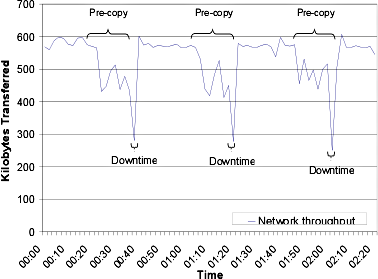
\includegraphics[width=0.9\linewidth]{images/vmware-network}
  \caption{Effekt von Live-Migraton auf das
    Netzwerk. Quelle:~\cite{nelson2005fast}}
  \label{fig:vmware-network}
\end{figure}

\subsection{Keine Ausfallzeit durch erzwungene Verschiebungen}
\label{sec:keine-ausfallzeit}
Neben den Anwendungsfällen zur Skalierung und Aufrechterhaltung von
(Cloud-)Services, gibt es ein weiteres Problem, mit dem international
agierende Anbieter umgehen müssen, und das sind die sich wandelnden
gesetzlichen Vorschriften zur Datenverarbeitung, die gerade in
Deutschland noch vielfach in Veränderung begriffen
sind~\cite{bdsg-2009}. Ein Beispiel ist Vorschrift, dass
personenbezogene Daten von deutschen Behörden nur auf deutschem Boden
verarbeitet werden dürfen. Diese Art von Gesetz schließt Dienste, die
in anderen Ländern große Datenverarbeitungsdienste bieten, oft von
Aufträgen deutscher Behörden aus. Rechenleistung in anderen Ländern
als Deutschland ist unter Umständen wesentlich billiger für ein
Unternehmen mit einem hohen Leistungsbedarf. Dauerhaft ein
Rechenzentrum in Deutschland zu betreiben, für die Möglichkeit, ab und
an einen Auftrag von einer deutschen Behörde zu erhalten, wiegt unter
Umständen nicht den Ertrag solcher Aufträge auf.

Durch die Möglichkeit, ohne Verlust des aktuellen Dienstzustandes die
Virtuelle Maschine umzuziehen, ist es jedoch möglich, solchen
gesetzlichen Vorschriften nichtsdestoweniger zu genügen. Indem der
Datenverarbeiter bei einem Cloud Hosting Service auf deutschem Boden
Rechenzeit einkauft, kann er den gestzlichen Vorschriften gerecht
werden. Die VMs, die für den Auftrag bereitgestellt sind, können
einfach in die Cloud auf deutschem Boden migriert werden. Migrationen
über Ländergrenzen hinweg, z.B. durch den Atlantik, sind zwar
notwendigerweise langsamer als zwischen Rechenzentren mit höherer
Lokalität, bei großen, lang laufenden Aufträgen ist das jedoch unter
Umständen zu vernachlässigen.

Auf diese Weise ist es Datenverarbeitungsdiensten möglich,
landesspezifischen Einschränkungen bezüglich der geografischen Lage
der physikalischen Nodes gerecht zu werden, und Services "`on-demand"'
anzubieten, ohne die Flexibilität von lokal vorbereiteten Maschinen
aufzugeben.

Die Amazon EC2 bietet diese Möglichkeit bereits zum Teil, indem man
solche Einschränkungen beim Kauf der Rechenzeit angibt. Derzeit müssen
dazu allerdings die VMs neu gestartet werden. Mithilfe von
Live-Migration könnte man hier einen Service anbieten, bei dem es
möglich ist, zur Laufzeit solche Einschränkungen zu konfigurieren,
ohne Downtime in Kauf nehmen zu müssen.

\subsection{Langzeit-Lauffähigkeit}
\label{sec:langz-lauff}
Das Versprechen der Cloud ist, Informationen und Dienste jederzeit
verfügbar zu haben, unabhängig von der physikalischen Verfügbarkeit
einzelner physikalischer Server oder Netzwerke respektive
Teilnetzwerke. Der Aufwand und damit die Kosten, die durch die
Umstellung bestehender Systeme (und der zugehörigen Prozesse)
entstehen, werden gerechtfertigt dadurch, dass der Zugang zu
kritischen Diensten und Informationen nicht alle paar Monate
unterbrochen wird, um mit den Folgen von
\begin{itemize}
\item Hardware-Ausfällen
\item Turnus-mäßigen Hardware-Upgrades
\item Schwankenden Anforderungen
\item Ausweitung des Kerngeschäfts
\item Hosting Wechsel
\end{itemize}
umzugehen.

In den obigen Anwendungsbeispielen kann diesen Problemen mit VM-Level
Live-Migration Technologie begegnet werden. Folglich ist die
Flexibilität von Cloud Hosting in Kombination mit dieser Technologie,
im Vergleich zum klassischen Rechenzentrum, in diesen Bereichen höher,
und besser an wechselnde Gegebenheiten anzupassen. Ein Anbieter kann
daher längerfristig davon ausgehen, dass Dienste und Informationen
verfügbar sind. Das vermindert den Druck und die Kosten, Dienste
"`In-House"' und Datensicherungen auschließlich "`vor Ort"' vornehmen
zu müssen. Geschäftsmodelle können daraufhin für größere
Marktschwankungen ausgelegt werden, ohne die Kosten für Hosting und
Hardware unnötig in die Höhe zu treiben. Weiterhin können strategische
Entscheidungen langfristiger getroffen werden, da die dauerhafte
Verfügbarkeit einfacher zu gewährleisten ist, und nicht mit längerer
Laufzeit rapide schwieriger und damit teurer wird.


%%% Local Variables:
%%% mode: latex
%%% TeX-master: "FelgentreffPape_2010_Live-MigrationInVirtuellenUmgebungen"
%%% End:
